%----------------------1----------------------------------------
\begin{frame}[t]{Conclusiones.}
    \begin{itemize}
        \item Las autoridades sanitarias del Paraguay no cuentan con datos computables que permitan a las comunidades científicas y académicas llevar a cabo actividades de investigación y análisis.
        %(1) Analizar nuevos métodos de muestreo de la abundancia poblacional del vector, con el fin de apoyar la lucha preventiva contra la enfermedad.

        %(2) Diseñar un modelo e implementar un sistema computacional mediante el cual se puedan procesar y presentar los resultados obtenidos, en un sistema de información geográfica.
        \item El enfoque SIG adoptado, permite realizar análisis complejos de la realidad espacial rápidamente.

        %(3)Diseñar el modelo de forma paramétrica y escalable, para que sea aplicable y extensible a cualquier región o área de estudio.

        \item El modelo y la herramienta resultante, son genéricos y extensibles, aplicables en cualquier región o área geográfica de estudio.

        %(4)Generar información relevante que pueda ayudar a las autoridades pertinentes para toma de decisiones en la lucha contra el dengue.
        \item Los mapas de interpolación permiten apreciar los niveles de infestación y el riesgo correspondiente a la abundancia de mosquitos.

    \end{itemize}
\end{frame}

\begin{frame}[t]{Conclusiones.}
    \begin{itemize}

        \item La construcción, instalación y recolección de puntos de control requiere trabajo de campo.

        \item La configuración del simulador del proceso evolutivo requiere de datos ecológicos.

        \item Los resultados obtenidos, utilizando configuraciones del material bibliográfico, son considerados una aproximación válida.

        \item Se pueden obtener mejores resultados ajustando las configuraciones con los datos ecológicos del Paraguay.

        \item El potencial analítico de la información generada es bastante amplio.

        \item En un futuro, con los ajustes y validaciones correspondientes a ser realizadas por expertos en el área, la información generada podrían permitir a las autoridades sanitarias a mejorar la planificación y lucha contra el dengue.
    \end{itemize}
\end{frame}

\begin{frame}[c]{Conclusiones.}
  \begin{center}
    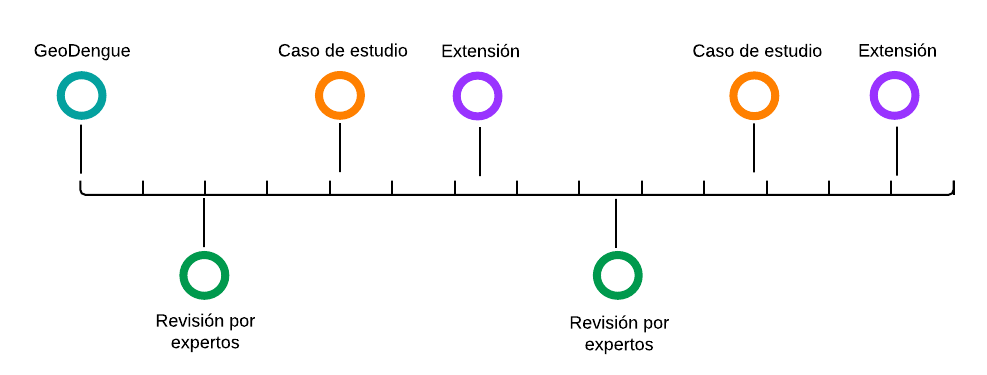
\includegraphics[width=\textwidth]{./graphics/linea-tiempo.png}
  \end{center}
\end{frame}

\begin{frame}[t]{Conclusiones.\\\textit{Cumplimiento de Objetivos.}}
    \begin{center}
        \begin{itemize}
        \item \textit{Analizar nuevos métodos de muestreo de la abundancia poblacional del vector, con el fin de apoyar la lucha preventiva contra la enfermedad.}
        \pause
        \\Si.
        \pause
        \item \textit{Diseñar un modelo e implementar un sistema computacional mediante el cual se puedan procesar y presentar los resultados obtenidos, en un sistema de información geográfica.}
        \pause
        \\Si.
        \end{itemize}
    \end{center}
\end{frame}


\begin{frame}[t]{Conclusiones.\\\textit{Cumplimiento de Objetivos.}}
    \begin{center}
        \begin{itemize}
        \item \textit{Diseñar el modelo de forma paramétrica, extensible y escalable, para que sea aplicable a cualquier región o área geográfica de estudio.}
        \pause
        \\Si.
        \pause
        \item \textit{Generar información relevante que pueda ayudar a las autoridades pertinentes para toma de decisiones en la lucha contra el dengue.}
        \pause
        \\Si.
        \end{itemize}
    \end{center}
\end{frame}
